\documentclass{standalone}

\usepackage{tikz}
    \usetikzlibrary{arrows.meta}
    \usetikzlibrary{calc}
    \usetikzlibrary{decorations.pathmorphing}

\tikzset{
    greensq/.style={
        green,
        fill=green!20, 
        line width=0.4mm,},
    redsq/.style={
        red,
        fill=red!20, 
        line width=0.4mm,},
    }
    
\begin{document}
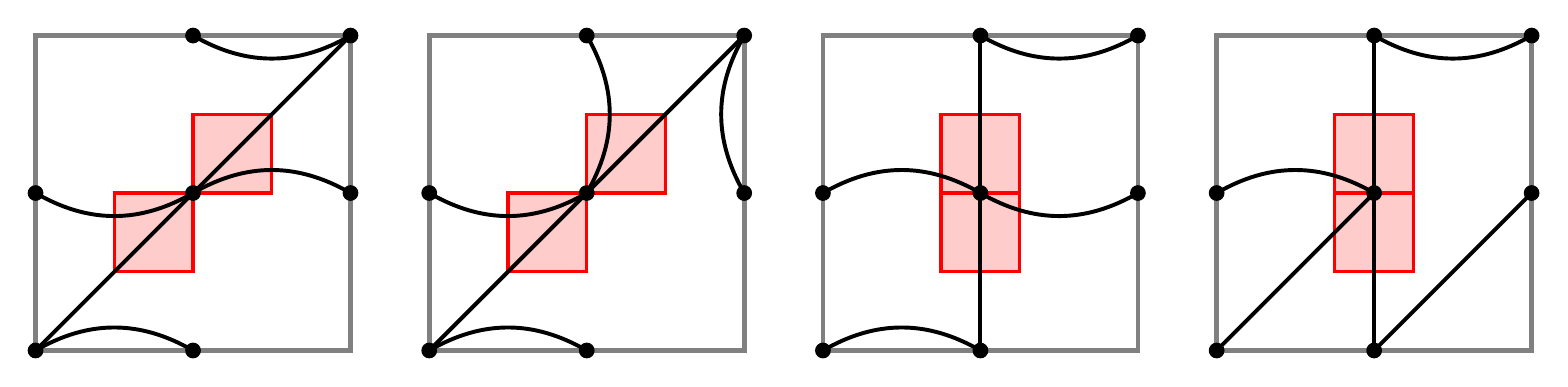
\begin{tikzpicture}
    % \draw[help lines] (0,0) grid (15,4);
    \foreach \x in
        {(0,0), (5,0), (10,0), (15,0)} 
        {\draw[black!50, line width=0.6mm] 
            \x rectangle+(4,4);}
    \foreach \x in
        {(1,1), (2,2), (6,1), (7,2), (11.5,1), (11.5,2), (16.5,1), (16.5,2)} 
        {\draw[redsq] \x rectangle+(1,1);}
    % \foreach \x in
    %     {(2,-5), (0,-3), (7,-5), (5,-3)} 
    %     {\fill[black!10] \x rectangle+(2,2);
    %      \draw[black!50, line width=0.6mm,] 
    %         \x++(0.3,0.3) -- +(1.4,1.4)
    %         \x++(0.3,1.7) -- +(1.4,-1.4)
    %         \x++(1,1)circle(0.5);}
    % \foreach \x in
    %     {(0,-5), (2,-3), (5,-5), (7,-3)} 
    %     {\draw[red, line width=0.6mm,] \x rectangle+(2,2);}
    \foreach \x in
        {(0,0), (2,0), (4,4), (2,4), (4,2), (0,2), (2,2)}
        {\fill[black] 
            \x circle (1mm)
            \x++(5,0) circle (1mm)
            \x++(10,0) circle (1mm)
            \x++(15,0) circle (1mm);}
    \path[line width=0.5mm]
        foreach \x in
            {(0,0), (2,2), (5,0), (10,0), (10,2), (15,2)}
            {\x edge[bend left] +(2,0)}
        foreach \x in
            {(0,2), (2,4), (5,2), (12,2), (12,4), (17,4)}
            {\x edge[bend right] +(2,0)}
        foreach \x in
            {(0,0), (2,2), (5,0), (7,2), (15,0), (17,0)}
            {\x edge +(2,2)}
        foreach \x in
            {(12,0), (12,2), (17,0), (17,2)}
            {\x edge +(0,2)}
        (7,2) edge[bend right] +(0,2)
        (9,2) edge[bend left] +(0,2);
    % \draw[line width=0.5mm]
    %     (0,0)--(4,4) 
    %     (0,2)..controls(1,1.4)..(2,2)
    %     (0,0)..controls(1,0.4)..(2,0)
    %     (2,2)..controls(3,2.6)..(4,2)
    %     (2,4)..controls(3,3.6)..(4,4);

\end{tikzpicture}
\end{document}